\section{Algebra}
\label{sec:algebra}

In this section we describe the operators of \tg algebra.  The algebra
is compositional --- all operators take a \tg or a pair of \tgs as
input, and produce a valid \tg as output.

\eat{ \tg algebra opertors come in two flavors.  The first are
  operations defined directly on the \rg representation, namely,
  analytics and temporal aggregation by change.  The second are
  operations such as selection and projection, which concern the
  structure of the elements of each representative graph --- its
  vertices, edges, and attribute values.  Some operators can be
  expressed (and computed) on both representations, and for such
  operators we give both semantics, and show that the result is
  equivalent.  Some operators, including \tg union, join and
  difference.... }

\subsection{Preliminaries}
\label{sec:algebra:prelim}

B\"ohlen et al.~\cite{DBLP:conf/vldb/BohlenSS96} show that temporal
selection, Cartesian product and difference all produce a coalesced
relation as output if the input was coalesced.  They also show that
temporal union and temporal projection can give rise to an uncoalesced
output even if the inputs were coalesced.  Intuitively, this is
because union and projection can give rise to duplicates in
traditional relational algebra, and lack of coalescing is the temporal
analogy to a duplicate.

These observations also hold in our scenario at the level of
individual relations, each containing representative graphs, vertices,
edges, or vertex/edge attributes.

Our algebra operates on \tgs, and so, in addition to keeping the data
structure (and its constituent parts) coalesced, we must ensure that
the result is a valid \tg.\eat{ This objective informed our design of
  the algebra, e.g., we did not include some flavors of temporal
  aggregation because the result would be invalid.  Further, this
  objective informs the rewriting of applicable operations over the
  \ve representation.}  Importantly, when manipulating the \ve
representation, we do not require that each intermediate state of the
data structure correspond to a valid \tg, but rather that the final
result, which is usually derived after several steps, be valid.  To
have a useful algebra, we do not reject a change that would lead to a
violation in referential integrity.  Instead, we compute a consistent
result by removing the tuples that violate referential integrity.

Consider a unary operation \op and suppose that it is being evaluated
over the \ve representation \op(\tve).  Algorithm~\ref{alg:op}
outlines the steps in the evaluation, overloading \opp as appropriate
when applying the operation to constituent parts of \tve.  Some of the
steps in Algorithm~\ref{alg:op} may be unnecessary because of the
properties of the particular operation, as we will see in the
remainder of this section.  Furthermore, some of the operations may
produce correct results (up to coalescing) {\em even when computing
  over uncoalesced inputs}.  This was discussed in the context of
temporal relational algebra in~\ref{DBLP:conf/vldb/BohlenSS96}, and
rules were proposed to eliminate superflous coalescing. We will
revisit this point in the context of \tg algebra when discussing lazy
evaluation in Section~\ref{sec:sys}.

\begin{algorithm}[h!]
\caption{Evaluation of a unary operation on \tve}
\begin{algorithmic}[1]
\REQUIRE \tg $\tve (\tv; \te; \tav; \tae)$, operation \insql{op}.\\
\STATE  $\tv' = \cl (\opp(\tv))$\\
\STATE  $\te' = \cl (\opp(\te))$\\
\STATE  $\tav' = \cl (\opp(\tav))$\\
\STATE  $\tae' = \cl (\opp(\tae))$\\
\STATE  enforce foreign keys on $\te'$ w.r.t. $\tv'$\\
\STATE  enforce foreign keys on $\tav'$ w.r.t. $\tv'$\\
\STATE  enforce foreign keys on $\tae'$ w.r.t. $\te'$\\
\RETURN new $\tve (\tv', \te', \tav', \tae')$\\
\end{algorithmic}
\label{alg:op}
\end{algorithm}

\subsection{Slice}
\label{sec:algebra:slice}

The unary {\em slice} operator, denoted $\xi_c (T)$, where $c$ is a
time period, cuts a temporal slice from $T$.  The resulting \tg will
contain representative graphs whose period $p$ has a non-empty
intersection with $c$ (i.e., $p$ is either contained within $c$ or
overlaps with it, see Section~\ref{sec:model:prelim}).  If $p.start <
c.start$ or $p.end > c.end$ for some tuple $(g, p)$, then $p$ is
trimmed to be within the boundaries of $c$: $\xi_c (\trg) = \{ (g, p
\cap c)~~|~~(g, p) \in \trg \wedge (\pred{c}{overlaps}{p} \vee
\pred{c}{contains}{p})\}$.

To evaluate $\xi_c (\tve)$, we apply $\xi_c$ to each of the four
constituent relations of \tve.  For example: 
$\xi_c (\tv) = \{ (v, p
\cap c)~~|~~(v, p) \in \tv \wedge (\pred{c}{overlaps}{p} \vee \pred{c}{contains}{p}) \}$, 
and analogously for each \te, \tav and \tae.

\eat{ 
In SQL, slice can be expressed as follows for $V$ (similarly for other
relations):}

\eat{\begin{small}
\begin{verbatim}
SELECT vid, a1, ..., an, greatest(estart, DATE ':date1'), 
       least(eend, DATE ':date2')
FROM V
WHERE eperiod OVERLAPS PERIOD (DATE ':date1', DATE ':date2')
\end{verbatim}
\end{small}}

{\bf Slice does not uncoalesce.} Whether evaluated over \trg or \tve,
slice is guaranteed to return a coalesced relation when evaluated over
a coalesced input.  This is because, for any relation \insql{R}, there
will be at most one tuple from \insql{R} in the result of $\xi_c (R)$,
with a validity period that is either the same as it was in \insql{R},
or further restricted (trimmed).  Therefore, there is no need to
coalesce \trg after slice, or on lines 1-4 of Algorithm~\ref{alg:op}
when operating over \tve.

{\bf Slice does not require FK enforcement for \tve.}  To see why,
consider an edge $\te(v_1, v_2, p)$ and one of the corresponding
vertices $\tv(v_1, p_1)$, such that $\pred{p_1}{contains}{p}$ (per
Definition~\ref{def:tg} condition~\ref{def:tg:c1}).  Suppose now that
slice was applied to \tv and to \te with condition $c$.  Is it
possible that edge $(v_1, v_2, p \cap c)$ is in the result of $\xi_c
(\te)$ (i.e., $p \cap c \neq \emptyset$), while vertex $\tv(v_1, p_1 \cap
c)$ is not in the result of $\xi_c (\tv)$ (i.e., $p_1 \cap c =
\emptyset$)?  Clearly, the answer is no, since
$\pred{p_1}{contains}{p}$, and so it must be the case that
$\pred{p_1}{contains}{(p \cap c)}$.  A similar argument justifies that
FK enforcement is not needed for $\xi_c(\tav)$ (w.r.t. $\xi_c (\tv)$) and
for $\xi_c(\tae)$ (w.r.t. $\xi_c (\te)$).

\subsection{Temporal subgraph matching}
\label{sec:algebra:subgraph}

Temporal subgraph matching is defined analogously to subgraph matching
in non-temporal graphs: it applies a subgraph function $f$ to every
representative graph of the input.  To ensure that a valid \tg is
computed as a result of this operation, we restrict our attention to
functions that compute a single subgraph of a given representative
graph as a result: $\sigma_f (\trg) = \{ (g', p)~~|~~(g, p) \in \trg
\wedge g' = f(g) \wedge$\\$V_{g'} \subseteq V_{g} \wedge E_{g'}
\subseteq E_{g} \}$.

\eat{For example, $f$ may select a subset of the vertices or edges of
  $g$ based on some condition that can be computed locally at a vertex
  or edge, or by a path / reachability expression.  In this paper we
  restrict our attention to conjunctive queries.}  Even more
specifically, we focus on functions that can be expressed as a pair of
{\em conjunctive queries} $\sigma_{Q_V,Q_E} (\trg)$, where $Q_V$
specifies {\em non-temporal predicates} over the vertices of $g$, and
$Q_E$ --- over the edges of $g$. (Computing arbitrary subgraphs of an
evolving graph is beyond the scope of this paper, and warrants a
deeper investigation, which we defer to future work.)

Like other unary operators, $\sigma_{Q_V, Q_E} (\tve)$ follows the
outline of Algorithm~\ref{alg:op}.  Importantly, since $Q_V$ and $Q_E$
may involve predicates over the attributes, we compute the join of the
vertex (resp. edge) relation with the corresponding attribute relation
to evalutate the query, and push selections as appropriate.  Line 1 of
Algorithm~\ref{alg:op} becomes: $\tv' = \pi_{v,p} (\sigma_{Q_{V1}} (V)
\bowtie \sigma_{Q_{V2}} (\tav))$.  Similarly, we compute $\te' =
\pi_{v_1,v_2,p} (\sigma_{Q_{E1}} (E) \bowtie \sigma_{Q_{E2}} (\tae))$
(line 2).  We compute $\tav' = \sigma_{Q_{V2}} (\tav)$ (line 3) and
$\tae' = \sigma_{Q_{V2}} (\tae)$ (line 4).

{\bf Subgraph does not uncoalesce \tve.}  Consider again the
computation of $\tv'$ described above, with a query that involves
projection, selection and join over temporal SQL relations $\tv$ and
\tav.  While selection and join cannot produce an uncoalesced output
if the input is coalesced, this is generally not the case for
projection, which may produce an uncoalesced
output~\cite{DBLP:conf/vldb/BohlenSS96}.  Interestingly, projection
also does not result in an uncoalesced output in this case. To see
why, suppose that $Q_V$ is trivial, i.e., that $\sigma_{Q_{V1}} (\tv)
= \tv$ and $\sigma_{Q_{V2}} (\tav) = \tav$. Then $\tv' = \pi_{v,p}
(\tv \bowtie \tav)$, and since $\tv \bowtie \tav$ is a primary
key-foreign key join, then $\tv' = \tv$.  If $Q_V$ is non-trivial,
i.e., $\sigma_{Q_{V1}} (\tv) \subset \tv$ or $\sigma_{Q_{V2}} (\tav)
\subset \tav$, then it will be the case that $V' \subset V$.  In both
cases, if $\tv$ is coalesced then so is $\tv'$.  A similar argument
applies to the edges relation $\te'$.  Finally, since \tav' and \tae'
are computed from coalesced input relations using selection, these
relations are guaranteed to be coalesced.  Thus, it is not necessary
to coalesce on lines 1-4 of Algorithm~\ref{alg:op}.

{\bf Subgraph does require FK enforcement for \tve.}  Perhaps the most
natural temporal subgraph query is one that specifies a selection
condition over the vertices, and computes the vertex-induced subgraph.
In this case we cannot compute $\te'$ from $\te$ alone, but will also
need to remove edges for which one or both vertices are not present in
$\tv'$ during the specified time period.  Similarly, we need to remove
tuples from $\tav'$ and $\tae'$ for which no corresponding tuples
exist in $\tv'$ and $\te'$, respectively.

{\bf Subgraph may uncoalesce \trg.} Consider the result of
$\sigma_{Q_V:{a.school='Drexel'},Q_E:\top} (\insql{T1})$ when applied
to the \tg in Figure~\ref{fig:rg}.  This query keeps vertices 1 and 3
in every representative graph, and no edges.  Since graphs
corresponding to time periods $p1$ through $p4$ will be identical, the
result will be uncoalesced, and will need to be coalesced explicitly.
The final result will consist of 2 representative graphs, with
vertices 1 and 3 for $[1/15, 7/15)$ and with vertex 3 for $[7/15,
    10/15)$.

\subsection{Temporal projection}%; vertex- and edge-map}
\label{sec:algebra:project}

\tg algebra supports a limited kind of projection: while key
attributes of vertices and edges must be retained, it is possible to
project out some or all non-key vertex and edge attributes.
$\pi_{\avv',\aee'} (\trg) = \{ (g', p)~~|~~(g, p) \in \trg \wedge
V_{g'} = V_{g} \wedge E_{g'} = E_{g} \wedge \avv' \subseteq \avv
\wedge \aee' \subseteq \aee \}$.  To evaluate projection over \tve, we
compute $\tav' = \pi_{\avv'} (\tav)$ and $\tae' = \pi_{\aee'} (\tae)$.

Because \avv and \aee are nested relations, it is natural to interpret
projection more broadly to mean {\em map}.  The user may specify an
arbitrary map function that is applied to each tuple in \avv
(resp. \aee), and transforms the properties of vertex $(v,p)$
(resp. of edge $(v_1,v_2,p)$).  In addition to removing properties, it
will often be useful to, e.g., flatten nested collections or reconcile
multiple values of the same property, e.g., compute a sum or an
average when map is invoked following temporal aggregation
(Section~\ref{sec:algebra:agg}), or temporal intersection or union
(Section~\ref{sec:algebra:join}).

{\bf Projection / map may uncoalesce \tav, \tae and \trg.}  Consider
\insql{T1} in Figure~\ref{fig:ve}, and suppose that we are computing
$\pi_{a:(name)} (\tav)$.  There will be two identical tuples in the
result for vertex $v_2$ for $[2/15, 5/15)$ and $[5/15, 10/15)$, which
    must be coalesced to return a valid \tav.  A similar argument
    holds for \tae. This operation will also produce two identical
    representative graphs in \trg in Figure~\ref{fig:rg} for $[2/15,
      5/15)$ and $[5/15, 10/15)$, which will have to be coalesced
        explicitly.

{\bf Projection and map do not require FK enforcement for \tve.}  This
is because, by definition of this operation, only \tav and \tae are
affected, while the contents of \tv and \te remain as in the input.

\subsection{Temporal aggregation}
\label{sec:algebra:agg}

We argued in the introduction that it is interesting and insightful to
analyze an evolving graph at different levels of granularity.  For
example, the user may want to aggregate multiple consecutive
representative graphs into a single representative graph, coarsening
the granularity, or to pre-define temporal resolution and look at the
graph at that scale, irrespective of whether this resolution happens
to be finer or coarse than the natural evolution rate of the graph.
For this, we will use temporal aggregation.  Our approach is inspired
by stream aggregation work of Li, et al.~\cite{Li2005}, adopted to
graphs, and by generalized quantifiers of~\cite{Hsu1995}.

The {\em temporal aggregation} operator is denoted $\gamma_{W,Q_V,Q_E}
(\trg)$, where $W$ is the window specification and $Q_V$ and $Q_E$ are
vertex and edge aggregation quantifiers.  

{\em Window specification} $W$ is of the form
$n~\{unit|\insql{changes}\}$, where $n$ is an integer, and $unit$ is a
time unit, e.g., $10~minutes$, $3~years$, or, more generally any
multiple of the usual time units (minutes, hours, days, weeks, months,
years).  Window specification of the form $n~\insql{changes}$ defines
the window in terms of change over \trg (which may be computed from
the \tve representation, see Section~\ref{sec:model:switch}).  For
example, $W=3~\insql{changes}$ will aggregate sequences of 3
representative graphs into 1.  Window boundaries are computed
left-to-right, starting with the least recent represenatative graph.
The right-most window may correspond to fewer than $n$ representative
graphs from the input.
%
Our window specification is similar to slide-by-row window in stream
aggregation~\cite{Li2005}.  Note that, because \tg algebra is
compositional, we do not support temporal aggregation with overlapping
windows. Also unlike~\cite{Li2005} we do not currently support
aggregation simultaneously by time and by non-temporal attributes
(e.g., vertex attributes). Incorporating this into \tg algebra and \ql
system is in our immediate plans.

{\em Aggregation quantifiers} $Q_V$ and $Q_E$ are of the form
\{exists | all | most | at least $n$ \}, where $n$ is a
decimal representing a ratio.  These are useful for producing
different kinds of representative graphs.  For example, to produce
representative graphs with only strong connections over a volatile
evolving graph, we may want to only include edges that span the entire
aggregtion window, or a large portion of the window.

Algorithm~\ref{alg:agg_ve} implements temporal aggregation over \tve.
We compute aggregation periods based on window specification in line
1.  Then, in lines 2-5 we assign a tuple from each \tv, \te, \tav and
\tae to one or several aggregation periods.  Next, as part of
$\gamma_{P,Q_V}(\tv)$ computation, we group vertices by $v$ and
evaluate $Q_V$ on each group.  Only groups for which $Q_V$ evaluates
to true are retained.  Edges are processed similarly by
$\gamma_{P,Q_E}(\te)$ on line 3.  Lines 4 and 5 compute
$\gamma_{P}(\tav)$ and $\gamma_{P}(\tae)$, respectively, by computing
a group for each vertex or edge within the period, and accumulating
all attribute values that correspond to a vertex or edge in a nested
collection.  It is possible but inconvenient to express the
aggregation operations on lines 2-5 in temporal SQL because each
vertex, edge or attribute tuple in the result of $\gamma_{P}$ may
belong to multiple periods.

\begin{algorithm}[h!]
\caption{Temporal aggregation in \tve.}
\begin{algorithmic}[1]
\REQUIRE \tve (\tv, \te, \tav, \tae), window specification $W$, vertex quantifier $Q_V$, edge quantifier $Q_E$.\\
\STATE $P = \ensuremath{computePeriods}(W, \tv, \te, \tav, \tae)$\\
\STATE  $\tv' = \cl (\gamma_{P,Q_V}(\tv))$\\
\STATE  $\te' = \cl (\gamma_{P,Q_E}(\te))$\\
\STATE  $\tav' = \cl (\gamma_{P}(\tav))$\\
\STATE  $\tae' = \cl (\gamma_{P}(\tae))$\\
\STATE  enforce foreign keys on $\te'$ w.r.t. $\tv'$\\
\STATE  enforce foreign keys on $\tav'$ w.r.t. $\tv'$\\
\STATE  enforce foreign keys on $\tae'$ w.r.t. $\te'$\\
\RETURN new $\tve (\tv', \te', \tav', \tae')$\\
\end{algorithmic}
\label{alg:agg_ve}
\end{algorithm}

\begin{figure*}
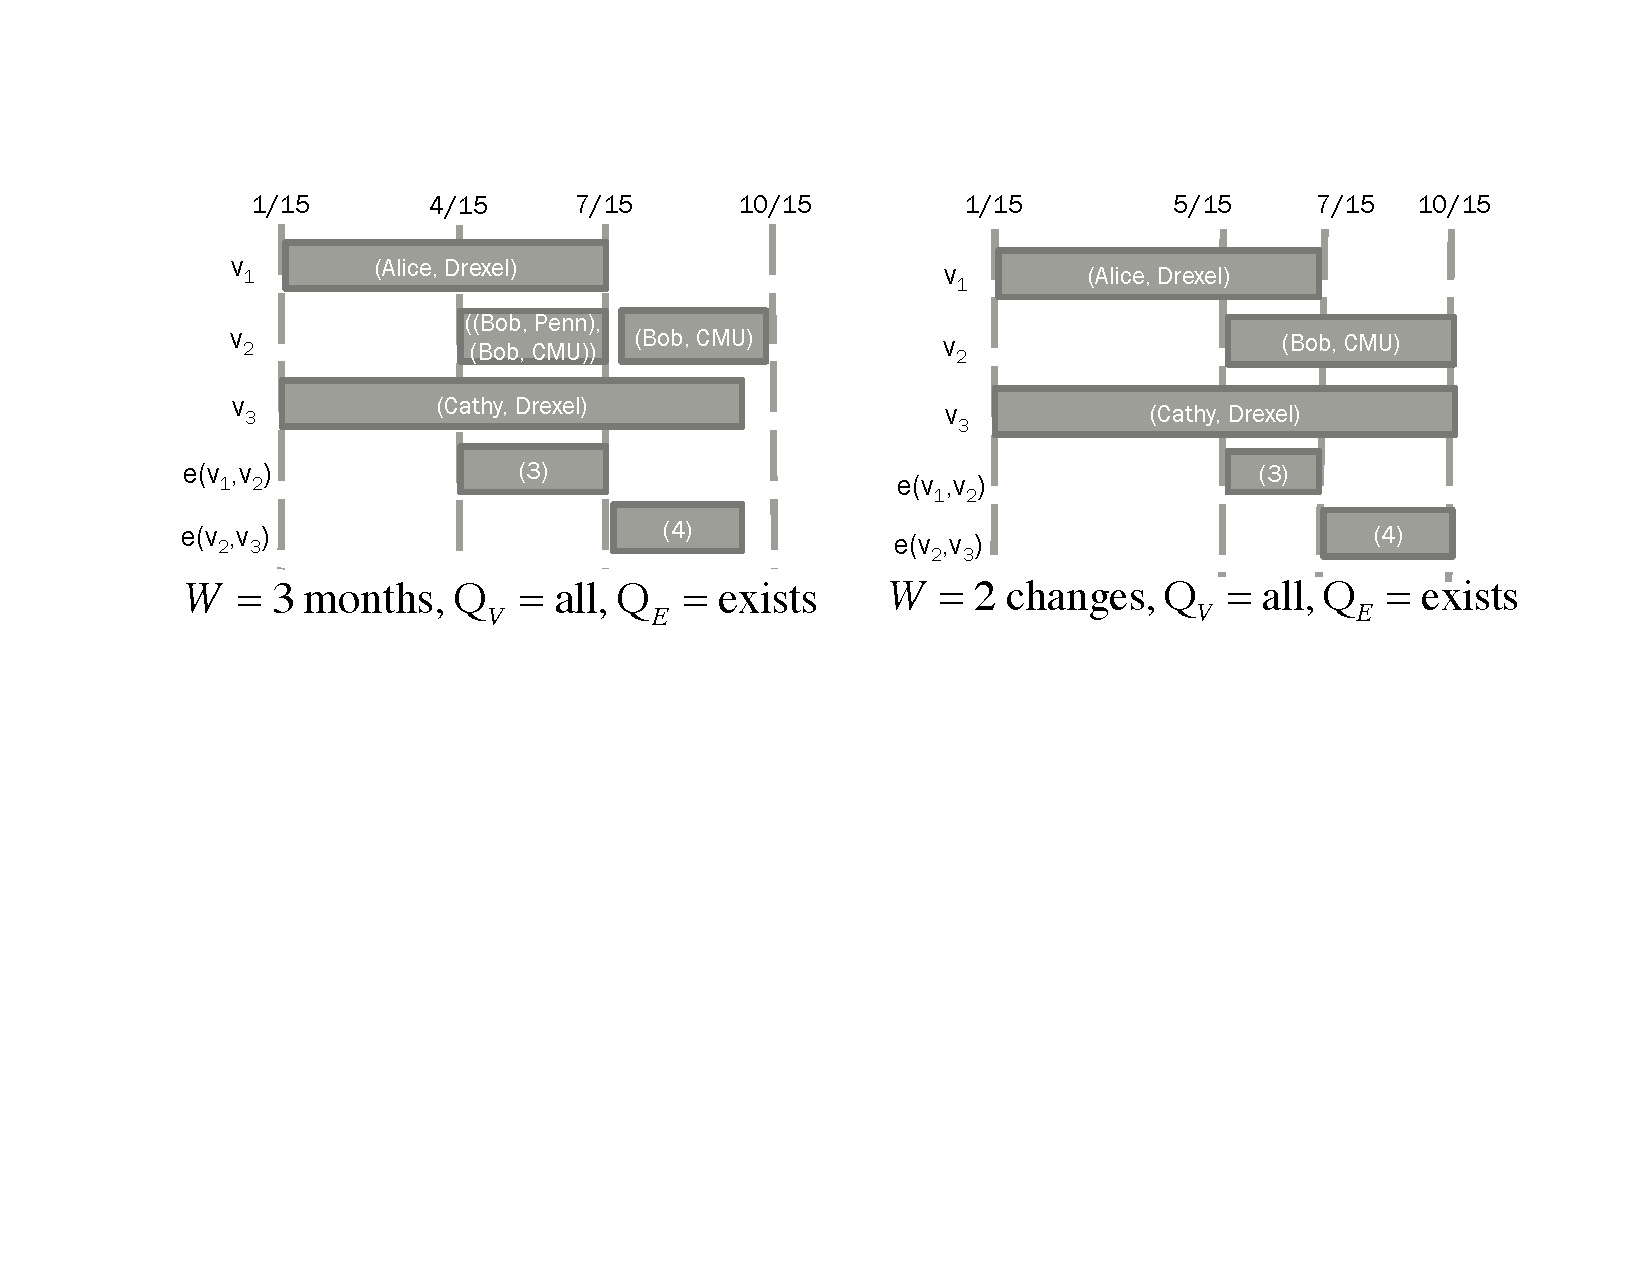
\includegraphics[width=5in]{figs/agg.pdf}
\caption{Temporal aggregation over \insql{T1} (Figure~\ref{fig:tg_ve}).}
\label{fig:tg_agg}
\end{figure*}

Figure~\ref{fig:tg_agg} illustrates Algorithm~\ref{alg:agg_ve} with
two examples, both applied to \insql{T1} of Figure~\ref{fig:tg_ve}.
The queries differ on their window specification (``3 months'' vs. ``2
changes'') but list the same aggregation quantifiers (``all'' for
vertices and ``exists'' for edges).  Note that$(v_2, [4/15, 7/15)$ is
  present in the result of $\gamma_1$ because $v_2$ exists for the
  entire period in the input \insql{T1}.  Further, because vertex
  properties took on values $(Bob, Penn)$ and $(Bob, CMU)$ during this
  period, both values are collected into the vertex attribute.  This
  is in contrast to only $(Bob, CMU)$ being associated with $v_2,
  [7/15, 10/15)$.

Next, consider the result of $\gamma_2$, and note that, while $v_2$
was present for part of $[1/15, 5/15)$, it was not there during the
  entirety of the period, and so is not included into the result
  (since $Q_V=all$).  Edge $e(v_1, v_2)$ is absent during $[1/15,
    5/15)$, because one of the vertices it connects ($v_2$) does not
    exist.

Temporal aggregation over \trg is computed by first calculating time
periods from $W$ and \trg, and then processing the representative
graphs directly.  Recall also that \trg can be computed from \tve (and
vice versa) as per Section~\ref{sec:model:switch}.


{\bf Temporal aggregation may uncoalesce \tve and \trg.} Consider a
\tg \insql{T} that consists of only 1 vertex $v_1$ and no edges, and
suppose that $v_1$ exists during the odd months of the year.  That is,
\tv contains $(v_1, [1/Jan/16, 1/Feb/16)), \ldots,$ $(v_1,
  [1/Nov/16,1/Dec/16))$, for which time periods do not meet and so
    these tuples cannot be coalesced.  Next consider $\tve'$ in the
    result of $\gamma_{W=2~months, Q_V=exists,Q_E=all}(T)$.  This
    relation will contain $(v_1, [1/Jan/16, 1/Mar/16)), \ldots,$
      $,(v_1, [1/Nov/16,1/Jan/17))$ --- one tuple per input tuple, all
        tuples meet and so \tv' must be coalesced.  A similar argument
        holds for other relations of \tve, and for \trg.

{\bf Temporal aggregation requires FK enforcement for \tve.}  As
illustrated in Figure~\ref{fig:tg_agg}, $(v_1,v_2,[1/15,5/15))$ is
  removed from $\te'$ not because it did not exist at some point
  during $[1/15,5/15)$ but because $(v_2,[1/15,5/15))$ is absent from
      $\tv'$.

\eat{ Our aggregation quantifiers are inspired by generalized
  quantifiers of~\cite{Hsu1995} with n-place delimiters.  $Q(R)$ as a
  Boolean-valued function of a relation''~\cite{Hsu1995}.  A
  quantifier contains an n-place determiner, e.g., ``at least one
  vertex in each window for each group'' is a 2-place determiner
  quantifier.  \tg algebra supports determiners from the set
  $\{at\ least\ one, all, most, at\ least\ n\}$, where $n$ is an
  integer representing a ratio.  $all$ is a usual universal quantifier
  that in standard SQL can be achieved with the use of two \insql{NOT
    EXISTS}.}

\eat{Aggregation in relational algebra produces results for each grouping
irrespective of how many results there are, unless a \insql{HAVING}
restriction is applied.  The quantification over the aggregation
results in evolving graphs is useful for producing different kinds of
representative graphs.  For example, to produce a representative graph
with only strong connections over a volatile evolving graph, we want
to restrict results to those edges that span the entire window or a
large subset of that window.  For this purpose we introduce
quantifiers.}

%%%%%%%%%%%%%%%%%%%%%%%%%%%%%%%%%%%%%%%%%%%%%%%%%%%%%%%%%%%%%%%%%%%%

\eat{
The second observation is that it is necessary to enforce referential
integrity.  Consider a pair of relations $R_i, R_j \in T_{VE}$, such
that there is a foreign key on $R_j$ referencing $R_i$, and consider
the couterparts of these relations $R'_i = \sigma_{c_i} R_i$ and $R'_j
= \sigma_{c_j} R_j$.  If the selection condition on $R_i$ is trivial
(i.e., $R_i = \sigma_{c_i} R_i$), then referential integrity will hold
on $R_i, R_j$.  However, if $c_i$ removes some tuples from $R_i$, then
it becomes necessary to idenfity tuples in $R'_j$ for which there is
no counterpart in $R'_i$ and delete them.}

\eat{
Recall that a \tg is a pair of coalesced temporal SQL relations, with
an integrity constraint that ensures that an edge exists at a time
when both vertices it connects also exist.  We start by investigating
the behavior of our model under a standard definition of temporal
relational algebra operators applied to $V$, $E$ or both in
Section~\ref{sec:algebra:rel}.  We then present the novel operations
of \tg algebra (Section~\ref{sec:algebra:graph}).  The main challenge
in both sub-section is understanding whether and when to coalesce $V$
and $E$, and how to efficiently enforce the integrity of the data
structure.}

%\subsection{Relational algebra operators over $V$ and $E$}

\eat{$V$ and $E$ are valid-time temporal relations, and we adopt (and
adapt) the semantics of period-based temporal
algebra~\cite{DBLP:conf/vldb/BohlenSS96} to our setting. }

\eat{1) Apply operation to V
2) Apply operation to E
3) Coalesce V if necessary
4) Coalesce E is necessary
5) Enforce integrity constraint}

\eat{Temporal selection $\sigma_c V = \{ \langle v, p, a_1, \ldots, a_n
\rangle | c(\langle v, p, a_1, \ldots, a_n \rangle) \}$ returns a
subset of the tuples in $V$. Note that the selection condition $c$ is
an arbitrary boolean condition that may also include predicates on
$p$.  }

\eat{When evaluated over coalesced input relations, temporal selection,
temporal Cartesian product and temporal negation preserve coalescing.}

\eat{
\begin{definition}[Selection]
Temporal and structural selection on $TG$ is a selection on the
attributes of $V$ and $E$, including entity periods.  $\sigma_{a
  \theta c}(TG)$, where $a$ are attributes of $V$ and/or $E$,
including periods, $\theta$ is a binary operation in the set $\{<,
\leq, =, \neq, \geq, >\}$, and $c$ is a value constant.
\label{def:selection}
\end{definition}}

\eat{Temporal and structural selection are supported by the same selection
operator and can be used together.  For example, one could select a
sub-graph in an evolving co-citation network of only authors whose
names start with letter A, over the past decade.  Because of the
constraint on $E$, even if the structural selection is only on
attributes of $V$, only edges connecting selected vertices are
retained.  Neither deduplication nor coalescing is required as a
post-operation.  Note that temporal selection and slice are different
because temporal selection does not modify entity periods, only
selects some of them.}

\eat{In SQL, selection can be expressed as a regular selection on V,
followed by a selection on E with integrity constraint enforced.}

\eat{\begin{definition}[Projection]
Projection on $TG$ is projection on attributes of $V$ and $E$ with
coalescing, i.e. \\$\Pi vid, p, a_1, \ldots, a_n(V); \Pi vid_1, vid_2,
p, b_1, \ldots, b_m(E)$. 
\label{def:projection}
\end{definition}}

\eat{\begin{definition}[Slice]
The unary operation \op{slice}, denoted $\sigma_{[start, end)}
  \insql{T}$ is a selection operation that includes...}

\eat{Slice on $TG$ is a selection on periods of $V$ and $E$ such that
$slice_{[a,b)}(TG) = \{t': t \in TG$, $t(p).overlaps(period(a,b)), t'
  = fit(t, period(a,b))\}$ and $fit(t, period(a,b))$ shortens the
  entity period $p$ to be within $[a,b)$.
\label{def:slice}
\end{definition}}

\eat{In SQL, slice can be expressed as follows for $V$
(similarly for $E$):}

\eat{\begin{small}
\begin{verbatim}
SELECT vid, a1, ..., an, greatest(estart, DATE ':date1'), 
       least(eend, DATE ':date2')
FROM V
WHERE eperiod OVERLAPS PERIOD (DATE ':date1', DATE ':date2')
\end{verbatim}
\end{small}}

%\subsection{Temporal aggregation}

\eat{Now that we have the window semantics and quantification defined, we
can define the aggregation operation over an evolving graph $TG$.}

\eat{It is often useful to analyze aggregate behavior of an evolving graph
over some coarser time period.  For example, a union of all
vertices/edges over 1 month is representative of that graph during
that month.  Analysis of aggregate behavior can lead to deeper insight
than of a snapshot.  For example, a co-authorship network DBLP is very
sparse --- one can only publish so many papers in any given month ---
on a daily or even monthly level of granularity, but can show
community formation and affiliation when aggregated over multiples of
years.  From this perspective, an evolving graph is a sequence of
representative graphs over consecutive arbitrary-length periods.}

\eat{
\begin{definition}[\tg Aggregation]
An {\em aggregation} operation over $TG$ is a function \\ $G_1, G_2,
\ldots, G_n, W, Q g f_1(A_1), f_2(A_2), \ldots, f_m(A_m)(TG)$, where
each $G_i$ is a grouping attribute from $TG$ with the exception of
$p$; $W$ is the window specification; $Q$ is a generalized quantifier
specification for vertices and edges on the coverage of the window;
each $F_i$ is an aggregation function; and each $A_i$ is an attribute
name from $TG$.
\label{def:agg}
\end{definition}}

\eat{This definition is similar to the regular relational algebra
aggregation definition, with the addition of the window specification
and the restriction of grouping attributes to exclude the time
periods.  However, both $V$ and $E$ relations are aggregated by the
same operation and the constraint on $E$ to contain only those
vertices that exist in $V$ is maintained.  The aggregation defined
this way allows to aggregate graphs structurally, temporally, or in
combination.  To aggregate only temporally, the grouping attribute
must be $vid$ for $V$ and $(vid1, vid2)$ for $E$.  To aggregate only
structurally, the window specification must be by 1 change.  Observe
that aggregation by 1 change with grouping by id is a no-op, and in
fact the sequence of representative graphs on the source data is equal
to the deduplicated sequence of snapshots.}

\eat{The quantifier is applied to the coverage of the window period
  within each grouping.  For example, to construct the persistent
  edges graph from the example above, we use the $all$ quantifier over
  the $E$ relation.  Only the edges that span the duration of the
  window period are produced.  Since the universal quantification is
  very restrictive, $most$ and $at\ least\ n$ quantifiers are more
  appropriate in some aggregations, especially over long windows.  To
  obtain a stable 1-month graph over an evolving network connections
  graph, we may ask for connections that exist in at least 90\% of the
  period.}

\eat{Remember that the schema for $V$ has a $(vid, p)$ primary key.  Any
aggregation operation must produce both a valid $vid$ and valid time
interval for each tuple.  We produce a $vid$ by using the hash of the
grouping variables to maintain temporal consistency.  The time
interval is produced by the window extent from the window
specification. Similarly for $E$.}

\eat{The aggregation functions over the selected graph attributes are used
to compute the new value representative of the whole window.  We
support the standard set $\{count, min,$ $max, sum, average\}$, as
well as $\{any, first, last, list\}$.  $first$ and $last$ refer to
first/last non-null value in the window and are possible because the
aggregating tuples have the time dimension, and the ties are decided
arbitrarily.  $count$ is the count of the number of distinct values
over the aggregation window.  Additional aggregation functions can be
defined by the user.}

\eat{\begin{figure*}
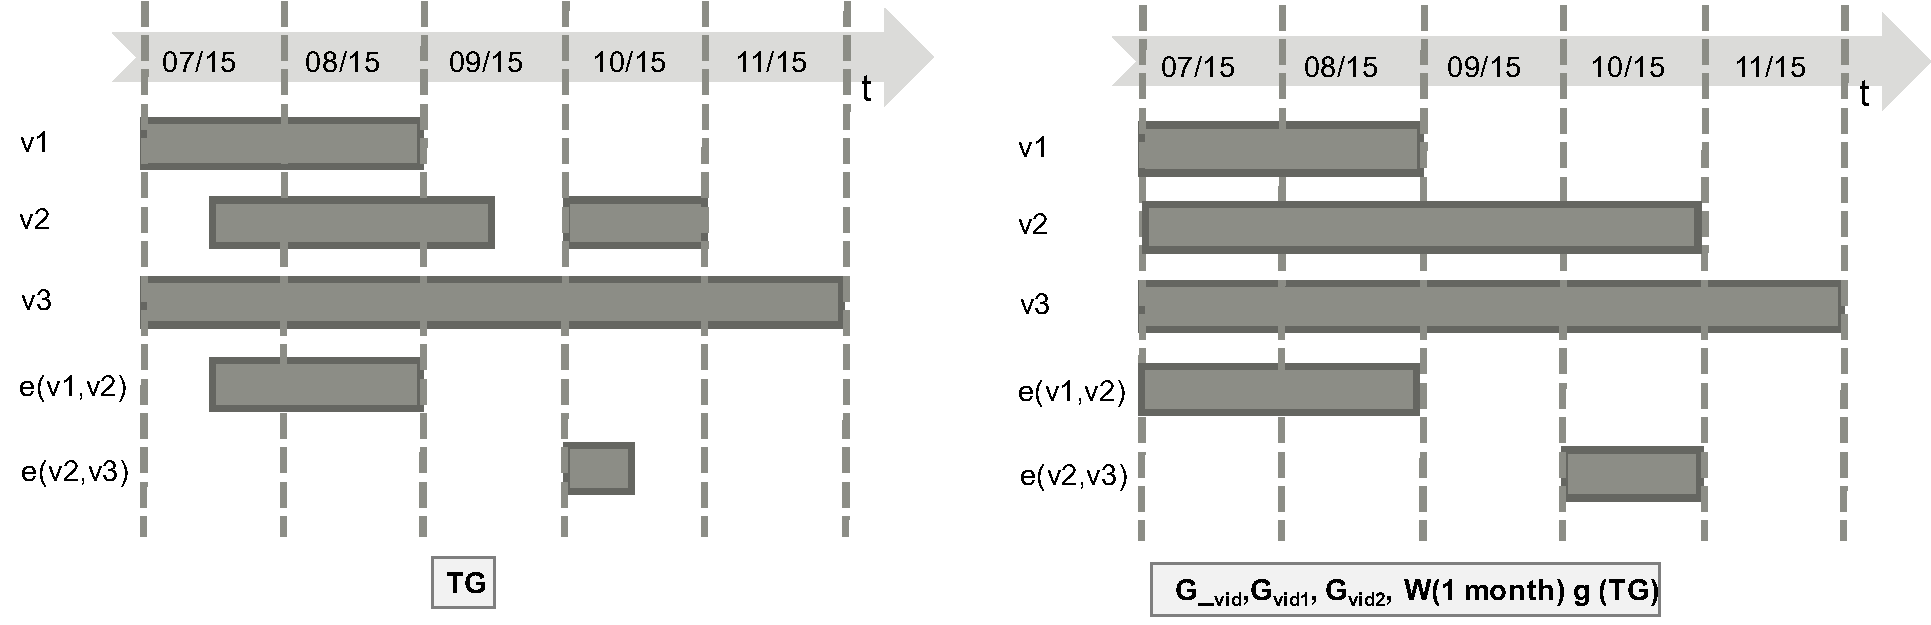
\includegraphics[width=6.5in]{figs/agg1.pdf}
\caption{1-month window aggregation with grouping by id, with
  existential vertex/edge quantifier.  Structure only.}
\label{fig:agg1}
\end{figure*}
}

\eat{An example in Figure~\ref{fig:agg1} shows a small \tg and a result of
aggregation by 1 month on that graph with $at\ least\ one$ quantifier,
with group by id.}


\subsection{Temporal union and intersection}
\label{sec:algebra:join}

\tg algebra supports two binary operations, temporal union and
intersection.

\eat{\begin{definition}[Union] Union of $TG1\ \cup\ TG2$ = $\{v, e: v
    \in TG1.V$ or $v \in TG2.V$ or $v(vid$, $f_1(a_{11}$, $a_{21})$,
    \ldots, $f_n(a_{1n}, a_{2n})$, $period(least(p_1, p_2),
    greatest(p_1, p_2)))$, $e \in TG1.E$ or $e \in TG2.E$ or $e(vid1,
    vid2, g_1(b_{11}, b_{21}), \ldots, g_m(b_{1m}, b_{2m})$,
    $period(least(p_1, p_2), greatest(p_1, p_2))) \}$, where each $f$,
    respectively $G$, is an aggregation function over one vertex,
    respectively edge, attribute where the values intersect over some
    period $p$.
\label{def:union}
\end{definition}}

\eat{\begin{figure*}
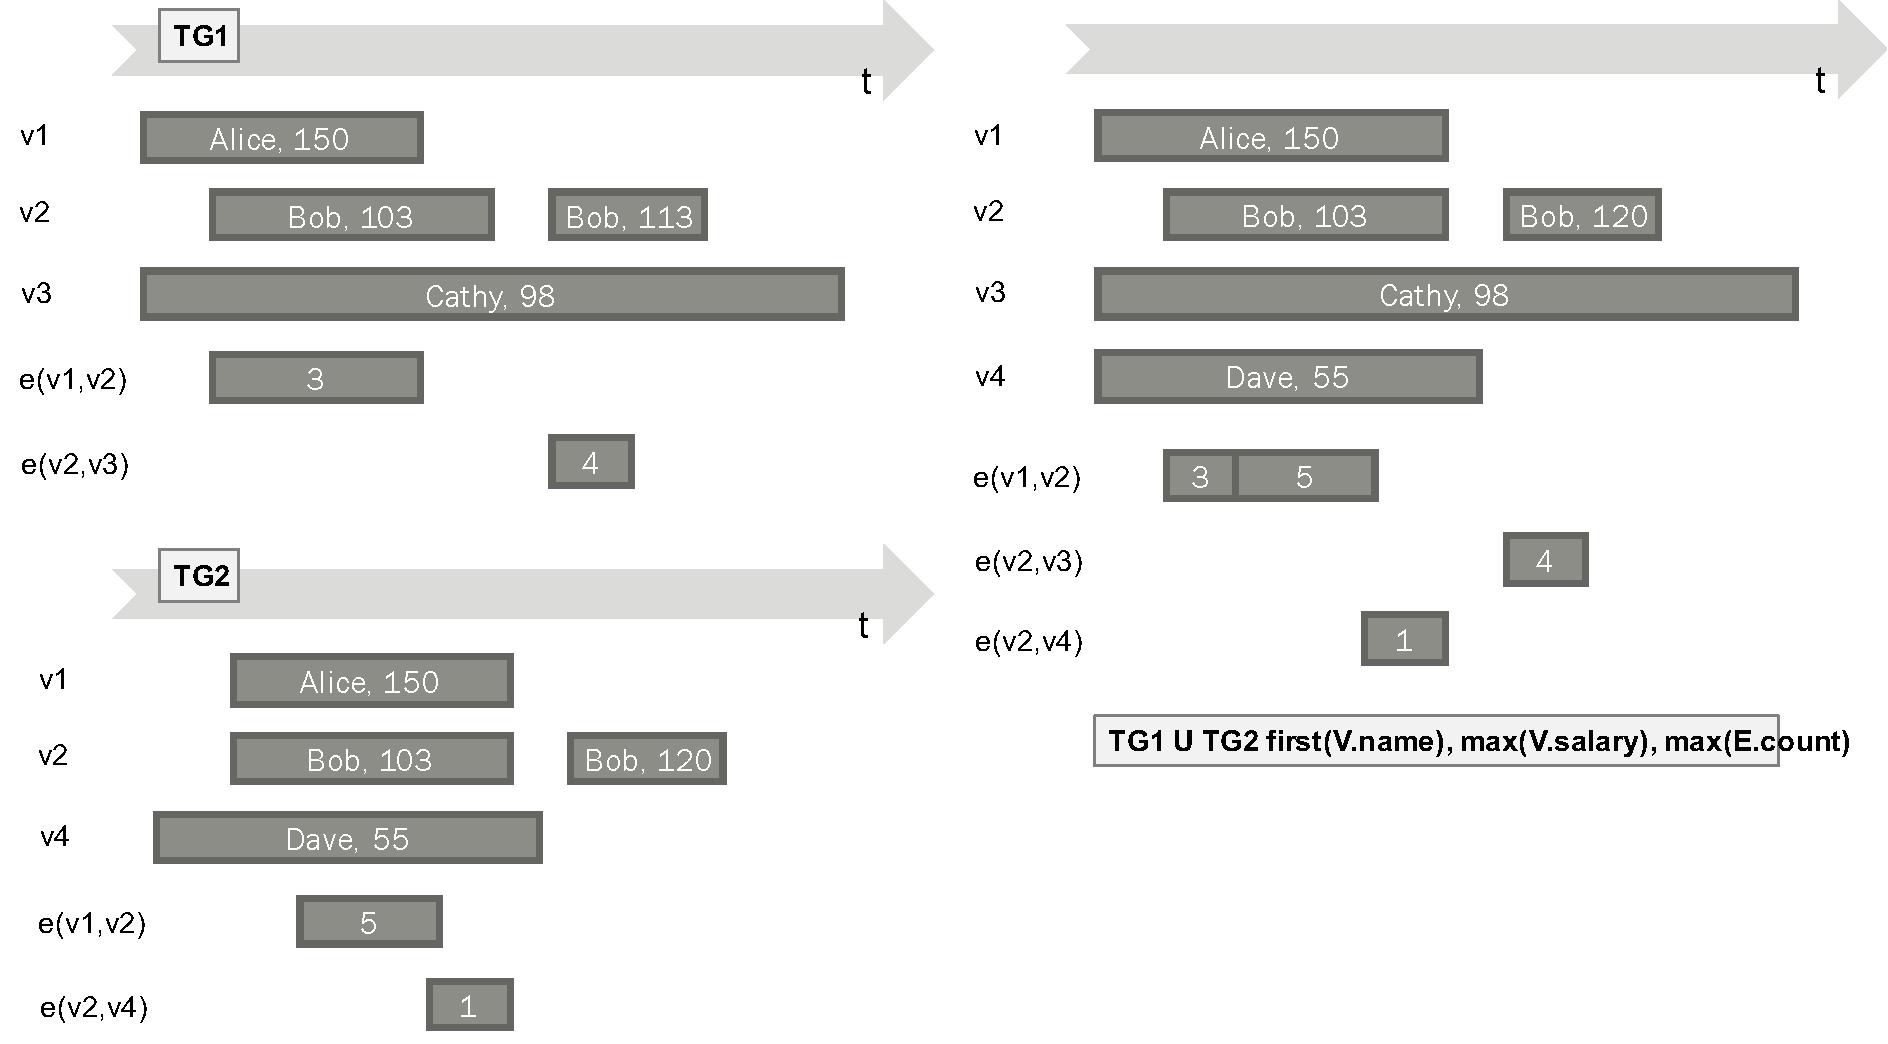
\includegraphics[width=6.5in]{figs/union.pdf}
\caption{Union of TG1 and TG2.}
\label{fig:union}
\end{figure*}}

\eat{In other words, union of two \tgs is simply all vertices and edges
from both \tgs, with vertex/edge attributes decided by specified
aggregation functions for each period where both values are present,
with coalescing.  Figure~\ref{fig:union} illustrates this concept.}

\eat{Similarly, intersection of two \tgs is an intersection of
vertices/edges of two graphs, with values for each overlapping
attribute computed by a specified aggregate function.}

